\begin{enumerate}
	\item Рассмотрим поисковые выдачи для для трех тестовых запросов. Число на каждой позиции 
	означает оценку релевантности для соответствующих документа и запроса по следующей шкале: 
	$4 = “perfect”, 3 = “excellent”, 2 = “good”, 1 = “fair”, 0 = “bad”$. Например, число $1$ 
	на позиции $5$ в первой выдаче означает, что документ на позиции $5$ релевантен первому 
	тестовому запросу на уровне $“fair”$.
	
	\begin{tabular}{ r | c | c | c }
		rank & query 1 & query 2 & query 3 \\
		\hline
		1 & 4 & 2 & 4  \\
		2 & 1 & 2 & 4  \\
		3 & 2 & 3 & 3  \\
		4 & 3 & 4 & 3  \\
		5 & 1 & 1 & 2  \\
		6 & 3 & 3 & 1  \\
		7 & 4 & 2 & 2  \\
		8 & 0 & 4 & 0  \\
		9 & 0 & 1 & 0  \\
		10 & 1 & 1 & 0 \\
	\end{tabular}
	
	Посчитайте среднее значение $F$-метрики и $MAP$. Считайте, что документы с оценками 
	релевантности $4$ и $3$ являются релевантными, а остальные (с оценками $0–2$)	
	нерелевантными. Также считайте, что для каждого из трех тестовых запросов общее число 
	документов с оценками $4$ и $3$ во всей тестовой коллекции равно $4$. Посчитайте среднее 
	значение $DCG@3$. В данном случае, используйте пятибалльной шкалу релевантности
	
	\begin{align*}
		&F = TODO \\
		&MAP = TODO \\
		&DGC@3 = TODO
	\end{align*}
	
	\item Выпишите формулу для метрики $ERR$. Дайте определение ее составляющим. Объясните 
	смысл каждой составляющей.
	
	\begin{equation*}
		ERR = \sum\limits_{k = 1}^{N}\frac{1}{k}\cdot P(PR = \frac{1}{k}) = 
		\sum\limits_{k = 1}^{N}\frac{1}{k}\cdot \varTheta^{k - 1}\cdot R_k \prod\limits_{i = 1}^ {k - 1}(1 - R_i) 
	\end{equation*}
	Составляющие:
	\begin{enumerate}
		\item $N$  
		\item $k$
		\item $\varTheta$
		\item $R_k$
		\item $P(PR = \frac{1}{k})$
	\end{enumerate}

	\item Назовите пять онлайн метрик. Объясните, как они отражают качество поиска. Для 
	каждой метрики приведите контрпример.
	\begin{itemize}
		\item \textbf{Abandonment}. Плохо, когда ничего не выбрал из выдачи и закрыл её. Он 
		увидел что его интересовало в кратком содержании
		\item \textbf{Time to last click}. Чем дольше чем позже был последний клик, тем 
		интереснее выдача. Либо пользователь ищет на этой странице хоть что-то подходящее 
		\item \textbf{Dwell time}. Если пользователь долго смотрит на выдачу, значит там 
		есть что-то интересное. Либо он просто не понимает, что на ней происходит
		\item \textbf{Time to first click}. Если пользователь быстро кликнул на ссылку, 
		значит он счет её релевантной. Либо элемент просто оказался на первой позиции, а его 
		по нему переходят чаще
		\item \textbf{Number of reformulations}. Если пользователю приходится 
		переформулировать запрос, значит он не нашел что искал. Либо он понял что искал 
		немного не то
	\end{itemize}
	
	\item $Multileaving$ – это метод оценки качества поиска (онлайн), аналогичный 
	интерливингу, но работающий с $n > 2$ различными выдачами. Выпишите алгоритм работы 
	мультиливинга. Каковы преимущества и недостатки мультиливинга по сравнению с 
	интерливингом?
	
	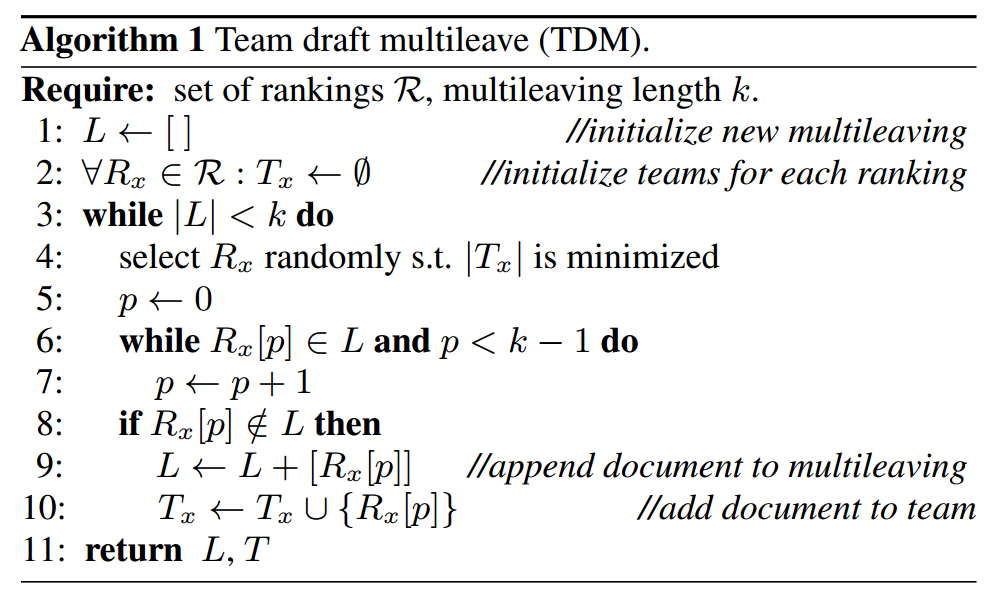
\includegraphics[scale=0.38]{ha/img/multileaving.PNG}
	
	\item Скорость сетевого соединения – $10MB$ в секунду. Каждая веб-страница занимает 
	$10KB$ и требует $500$ миллисекунд для загрузки. Сколько нужно запустить параллельных 
	потоков для обхода веба, чтобы полностью использовать возможности сетевого соединения?
	\begin{equation*}
		\frac{10MB}{10KB} = 1024
	\end{equation*}

	Кроме того, обходчик веба должен делать паузу в $10$ секунд между загрузками с одного и 
	того же веб-сервера. Сколько различных веб-серверов в минуту должен обходить кроулер, 
	чтобы полностью использовать возможности сетевого соединения?
	\begin{equation*}
		10 \cdot 1024 = 10240
	\end{equation*}

	\item Рассмотрим систему поиска по электронным книгам с точки зрения контент-провайдера и 
	с точки зрения разработчиков поисковика
	
	\begin{enumerate}
		\item Вы владеете электронной библиотекой и зарабатываете на предоставлении доступа к 
		каждой конкретной книге. Вы хотите, чтобы пользователи могли находить книги из вашей 
		библиотеки с помощью сторонних поисковых систем, но чтобы доступ к книгам 
		предоставлялся только через ваш веб-сайт. 
		
		\begin{itemize}
			\item Какими способами вы можете упростить работу с вашими данными для 
			разработчиков поисковиков?
			\begin{itemize}
				\item Предоставить API для метаданных
				\item Позволить индексировать файлы, но не сохранять в кэш
			\end{itemize}
			\item Как вы можете обезопасить себя от несанкционированного доступа к вашим 
			данным?
			\begin{itemize}
				\item Настроить firewall
				\item Установить большой таймаут между запросами
				\item Отключить индексирование/запретить кэширование файлов роботами
			\end{itemize}
		\end{itemize}
		 
		\item Вы разрабатываете поисковик по электронным книгам
		\begin{itemize}
			\item Какими целями вы, в первую очередь, будете руководствоваться при сборе 
			данных: объем, качество, свежесть (т.е. соответствие между вашей версией 
			документа и его онлайн версией)?
			
			\textit{Решение. }В порядке убывания важности:
			\begin{enumerate}
				\item Качество. Лучше меньше книг, но хорошо структурированных с рабочим поиском.
				\item Объем. Поиск ненужен, если книг мало
				\item Свежесть. Содержание уже написанных книг меняется редко, обычно в таких случаях появляется новая редакция $\Rightarrow$ проблема решится предыдущими двумя пунктами
			\end{enumerate}
			\item Какими способами вы будете собирать данные и почему?
			\begin{itemize}
				\item API
				\item Открытыми источниками с книгами
				\item Crawling других сайтов с книгами
			\end{itemize}
			\item Вы можете загружать 1000 книг в день. Каким образом (приблизительно) вы 
			распределите эту квоту между загрузкой новых книг и обновлением уже загруженных и
			почему?
			\textit{Решение.} 980/20. см пункт "свежесть"
		\end{itemize}
	\end{enumerate}
	
	\item  Как удаление стоп-слов и лемматизация влияют на размер индекса? Дайте	
	развернутый ответ.
	
	\item Какую минимальную информацию должен содержать индекс, чтобы обрабатывать запросы с 
	булевыми операциями? Какую информацию нужно добавить в индекс, чтобы документы можно было 
	ранжировать по их “похожести” на запрос (используйте определение “похожести”, которое вам 
	кажется разумным). Дайте развернутый ответ
\end{enumerate}
